\section{Semantics theory}\label{sec:semantic}
\emph{''Programming language semantics is the study of mathematical models of and methods for describing and reasoning about the behaviour of programs.''}\cite{transtrees}\\
The citation above sums up the whole meaning of semantics. In other words; programming language semantics give a formal description of program execution.

Two forms of operational semantics are generally used when describing program behaviour, \emph{big-step} and \emph{small-step}.
Big-step semantics describe an entire computation in a single transition;
$ \gamma \rightarrow \gamma' $.
Where $\gamma'$ is always a terminal configuration.
Small-step semantics describe a single step of a larger computation in a transition; $ \gamma \Rightarrow \gamma' $. Where $ \gamma' $ is not necessarily a terminal configuration.

Both have their pros and cons, big-step semantics are easier to formulate than the other, sacrificing details in the process and not being able to describe non-terminating programs. Small-step semantics can be complex to formulate and in contrast to big-step, have detail and describe all types of programs, terminating and non-terminating.\cite{opsemantics}\cite{transtrees}

\subsection{Environment-store model}\label{subsec:env-sto}
The semantics of \langname{} are described with the help of the environment-store model. The model describes how variables are bound during program execution. Each variable is bound to a storage cell, and the content of the storage cell is the value of the variable.

The below example is a visual representation of the environment-store model and how it works. The difference between this one and the \emph{''state''- model} is that the environment-store model provides more details as to where changes take place during execution.
\begin{figure}[!h]
\centering
	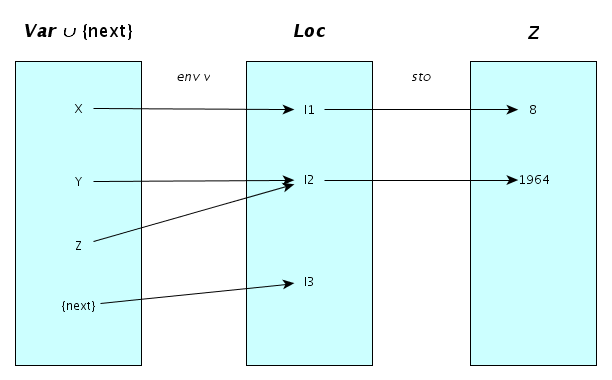
\includegraphics[scale=0.55]{img/envstore.png}
	\caption{Example of a variable environment and a store \cite{transtrees}}
	\label{img:env}
\end{figure}\\
In Figure \ref{img:env}, there are three variables plus a reference called \texttt{\{next\}}, which always points to the next available location. What cannot been seen is the function \texttt{new}, that for every location returns its successor, whether it is available or not.
\begin{description}
\item Variable $X$ is bound to location $l_1$, which points to a store containing the integer '8'.
\item Variable $Y$ is bound to location $l_2$. which points to a store containing the integer '1964'.
\item Variable $Z$ is bound to location $l_2$ like $Y$ is, the location points to the same integer as before.
\item Reference \texttt{\{next\}} is bound to location $l_3$, as it is not bound to any variable and therefore is unassigned.
\end{description}
%\\\\
As mentioned before this model provides more detail. When data changes, the store is updated to \emph{store'} and when changes within an environment happen, the environment is updated to \emph{environment'}. This is opposed to ''state''- model where the state is updated to \emph{state'} to indicate all changes.